\section{Introduction}
\label{sec:db:intro}


This chapter describes a procedure for searching for a dark boson, \db, of
unknown mass and lifetime\footnote{
  Throughout this chapter, the symbol \db shall denote a general dark boson and all references to
  a \Kstarz will be implicitly referencing the $K^*(892)^0$; unless explicitly stated otherwise.
}.
A frequentist method is applied to the dimuon distribution of \btokstrmumu candidates,
to search for an excess of events above the \sm background, consistent with a \db decaying into a
pair of muons.
Lifetime information is added by
splitting candidates into two bins of decay time: those which are prompt, and the \db vertex is the
same as the \Kstarz vertex; and
those which are displaced.
%searching for an excess of dimuon candidates in two bins of decay
%time:
%one prompt, and one displaced.


%Chapter~\ref{ch:theory} explains that the \sm cannot explain \dm, which is evidenced by
%numerous experimental observations.
Chapter~\ref{ch:theory} explains that the \sm cannot explain
the
numerous experimental observations of \dm.
Little is known about dark matter, except that it interacts gravitationally, and does not interact
with electromagnetic radiation to any significant extent.
A possible extension to the \sm is to introduce a dark sector, which can contain a rich variety of
distinct particles operating through forces that are hitherto unknown.
Dark sector particles would be gauge singlet states with respect to the \sm, and
only be able to communicate with known particles via weakly interacting messenger particles
through one of four \emph{portals}: the vector, axion, Higgs, and neutrino
portals~\cite{Essig:2013lka}.
Interaction terms for messengers in each of these portals are given in
\Table{tab:db:overview}.
%In many dark sector models, the \dm is observable because there
%is some mixing between the \db and an \sm particle.
%In most dark sector models, the only way that a \db can be observed is if it mixes with a \sm
%particle, and the superposition of the two states decays into, in this case, a dimuon pair.

Theories involving dark sectors are tremendously attractive because it is relatively easy to
construct a complex theory that explains various unexplained phenomena.
Yet, these can have little impact on the \sm observables since the interaction between the two
sectors can be extremely weak.

\begin{table}
  \caption[Summary of dark boson portals]
  {
    %from 1311.0029
    A summary of portals through which a new dark boson could operate, as given in
    Ref.~\protect\cite{Essig:2013lka}.
    Terms are defined as:
    %$F_{\mu\nu}$ is the Yang-Mills field;
    $F_{\mu\nu}$ is the field strength tensor of the photon;
    $F^\prime_{\mu\nu}$ is the dark photon field;
    $\epsilon$ characterizes mixing between the \sm and the dark photon;
    $f_\db$ is scale at which Peccei-Quinn global $U(1)$ symmetry is spontaneously broken;
    $G_{\mu\nu}$ is the gluon field strength tensor;
    $S$ is a dark scalar field with coupling strengths $\mu$ and $\lambda$ to the Higgs field;
    and the sterile neutrino couples to a $H$ with a strength $Y_N$.
  }
  \label{tab:db:overview}
  \begin{center}
    \begin{tabular}{llccc}\toprule
      \cellc{Portal} & \cellc{Particles} & \multicolumn{3}{c}{Operator(s)}
      \\\midrule
      Vector & Dark photons && $-\tfrac{\epsilon}{2\cos\theta_W}F_{\mu\nu}F^{\prime\mu\nu}$ \\
      Axion & Pseudoscalars & $\tfrac{\db}{f_\db}F_{\mu\nu}\widetilde{F}^{\mu\nu}$
      & $\tfrac{\db}{f_\db}G_{i\mu\nu}\widetilde{G}^{\mu\nu}_i$
      & $\tfrac{\partial_\mu \db}{f_\db}\xbar{\psi}\gamma^\mu\gamma^5\psi$ \\
      Higgs & Dark scalars && $(\mu \db + \lambda \db^2)H^\dagger H$ \\
      Neutrino & Sterile neutrinos && $Y_N\ell H\db$ \\
      \bottomrule
    \end{tabular}
  \end{center}
\end{table}


The Higgs portal has a scalar messenger particle which can mix with the \sm Higgs.
There are a number of models which incorporate a scalar messenger particle that interacts with the
Higgs.
One class of models incorporate an \emph{inflaton}, which is the quanta of the hypothesised
inflaton field responsible for the inflationary period of the Universe; beginning around
$t=10^{-36}\sec$.
%shows the Higgs-inflaton mixing angle as a function of inflaton mass.
Figure~\ref{fig:db:inflaton} shows the allowed parameter space of the mixing angle between the \dm
and Higgs, $\theta$, as a function of mass.
it is possible that inflatons are light, in the range
$270<\mass{\db}<10^{4}\mev$~\cite{Bezrukov:2009yw}, and might therefore be accessible in the decay
\btokstrdb.
These models also help to solve other problems, such as the
%the Higgs hierarchy problem and explain the
\BAU~\cite{Hertzberg:2013mba,Hertzberg:2013jba}.

%Reference~\cite{Bezrukov:2009yw} considers inflatons with masses in the range
%$1<\mass{\db}<1000\mev$ with lifetimes in the


\begin{figure}
  \begin{center}
    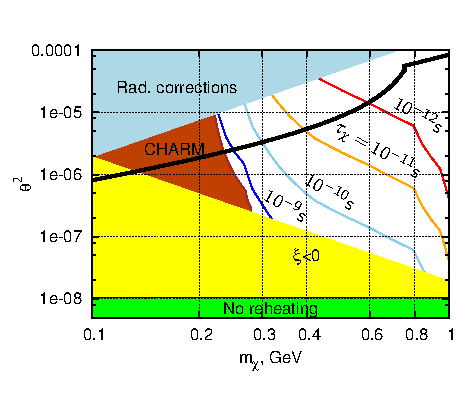
\includegraphics[width=0.6\textwidth]{mchi_theta_dm_labels}
    \caption[Parameter space for a model including an inflaton]
    {
      Allowed and excluded regions of the Higgs-inflaton mixing parameter squared as a function of
      inflaton mass, taken from Ref.~\protect\cite{Bezrukov:2014nza}.
    }
    \label{fig:db:inflaton}
  \end{center}
\end{figure}



%High energy \lhc experiments at the \lhc have put stringent limits on new $U(1)$ states under the
%assumption that the coupling of \darkgamma to \sm states is large.
%However, if the coupling of these states is weak then \darkgamma could be light.

Chapter~\ref{ch:theory} introduces the idea of \gls{PQ} symmetry breaking leading to an axion
which resolves the strong \CP problem.
Unlike other dark boson portals, the axion portal introduces a term in the Lagrangian which couples
messenger axions to fermions directly.
In order for the axion portal to couple to a dark sector containing TeV-scale \dm, the messenger
particles are predicted to have a mass in the range $360<\mass{\db}<800\mev$ and a decay
constant in the range $1\lesssim f_\db\lesssim3\tev$~\cite{Nomura:2008ru}.
Figure~\ref{fig:db:feynman} shows a Feynman diagram of how the decay \btokstrdb might proceed;
it shows an \fcnc where the \db results from a coupling to a \tquark quark.
Therefore, searching for evidence of a \btokstrdb where \dbtomumu is particularly sensitive to
portals which couple strongly to mass, as is the case for axions.

\begin{figure}
  \begin{center}
    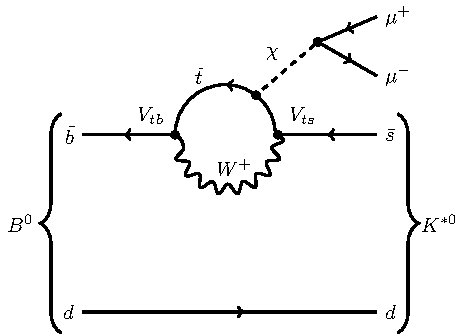
\includegraphics[scale=1]{feynman_inf}
    \caption[Feynman diagram for the decay \btokstrdb]
    {
      Feynman diagram showing the decay \btokstrdb, and \dbtomumu.
      Depending on the portal through which the \db acts, it couple directly to the muons, or need
      to mix with a \sm Higgs, $Z$, or photon.
    }
    \label{fig:db:feynman}
  \end{center}
\end{figure}

It is known that \sm would be a gauged field theory, and it is therefore reasonable to assume that
the dark sector is also gauged, but under a different group.
If this were to be the case, the \sm $U_Y(1)$ generator could kinetically mix with with generator
of the dark $U(1)$ group, giving rise to a particle, often called a \emph{dark photon}, interacting
through the vector portal.
%Figure~\ref{fig:db:darkphotonlimits} shows the existing parameter space for the mass of a dark
%photon depending on the value of the mixing parameter $\epsilon$; for $\epsilon\lesssim10^{-3}$ the
%mass of the dark
%photon could be in the range $2m_\mu<\mass{\db}<1000\mev$~\cite{Essig:2013lka}, which is accessible
%with the following analysis.

%\begin{figure}
  %\begin{center}
    %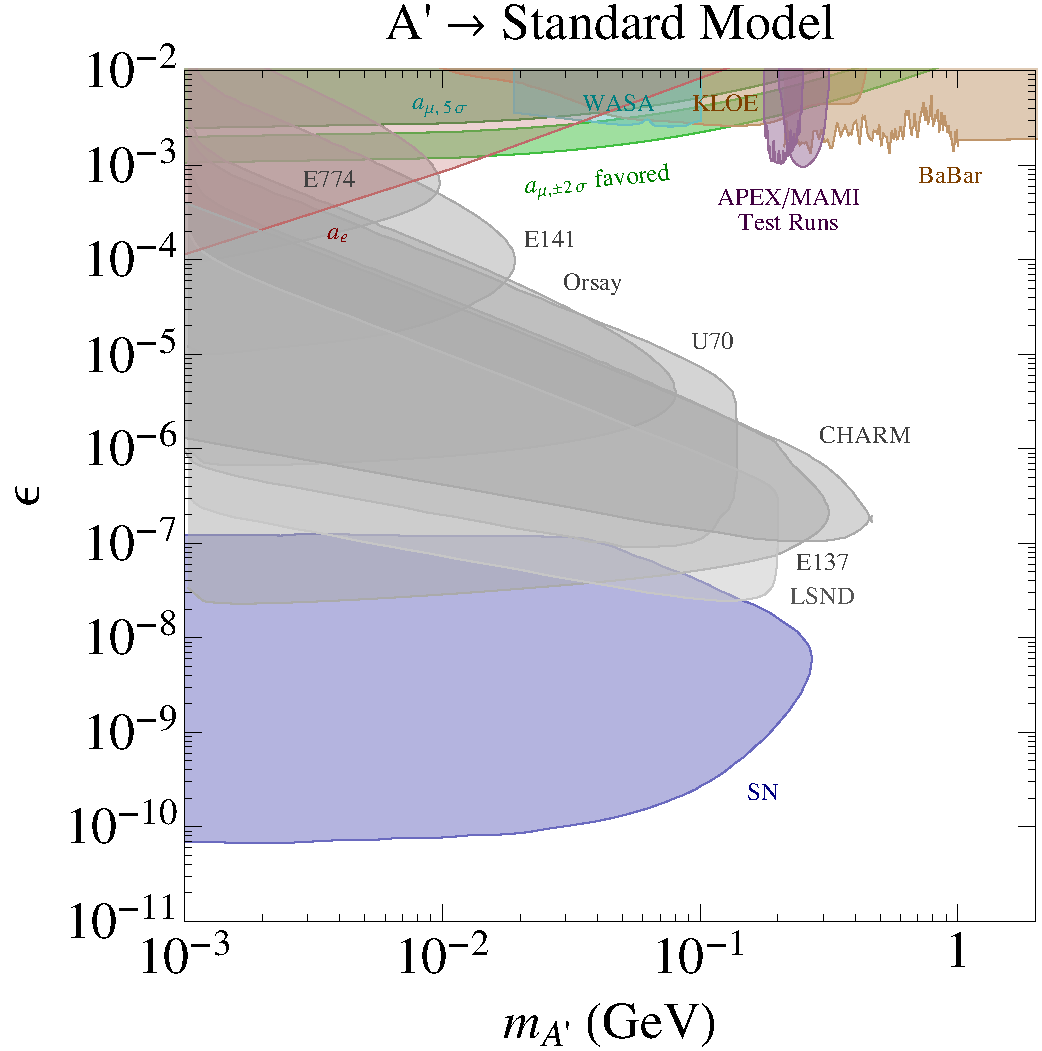
\includegraphics[width=0.48\textwidth,trim=0 0 0 1.8em,clip]{A-visible-large}
    %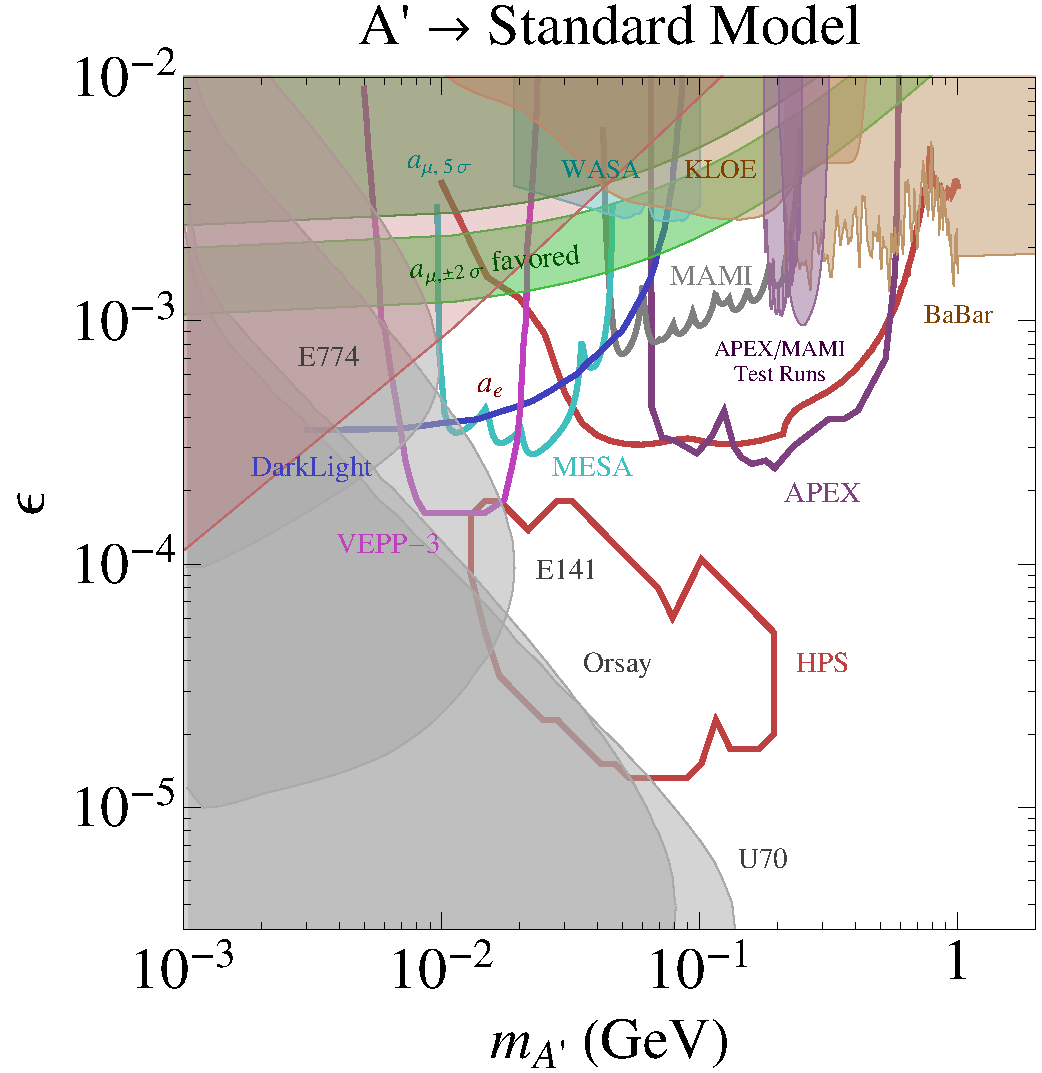
\includegraphics[width=0.48\textwidth,trim=0 0 0 1.8em,clip]{A-visible-zoom}
    %\caption[Paramter space for a model including a dark photon]
    %{
      %Parameter space for dark photons, $A^\prime$, with a mass above $1\mev$ showing the $90\pc$
      %confidence level limits from numerous experiments.
      %The right-hand panel is a zoom in of the left-hand panel, at low $\epsilon$; where
      %the parameter $\epsilon$ characterizes the mixing between the \sm photon and the
      %dark photon.
      %These plots are taken from Ref.~\protect\cite{Essig:2013lka}.
    %}
    %\label{fig:db:darkphotonlimits}
  %\end{center}
%\end{figure}
In principle, the following analysis is sensitive to any dark sector particle.
Practically, other experiments have searched directly for dark bosons with mass independent
couplings using much larger data samples.
For example, the NA48/2 collaboration has searched for a dark photon directly in the decay
\decay{\piz}{\gamma\darkgamma}~\cite{CERNNA48/2:2015lha}, and the \babar collaboration have
searched for evidence in the decay $\decay{\ee}{\gamma\darkgamma}$~\cite{Lees:2014xha}.
The coupling here is mass independent, and therefore this search is less sensitive to dark photons
in comparison to these direct production searches.


\SUSY could also be restricted, at energies reached thus far, to a dark sector.
%There are numerous mechanism through which a messenger particle might communicate with the \sm, one
%way is via the Goldstone bosons associated with the broken gernerators of \SUSY.
It is known that \SUSY is a broken symmetry and thus must have associated Goldstone particles:
a fermionic \emph{goldstino} and associated super-partners called \emph{sgolditinos}, which are
scalar and pseudoscalar.
In some models, the sgolditinos are the messenger particles between the \sm and the dark \SUSY
sector.
After \SUSY breaking, the goldstino becomes the longitudinal component of the gravitino, and the
sgoldstinos are massless particles, which gain mass from corrections at higher orders.
Then, after electroweak symmetry breaking, these sgoldstinos interact with \sm fermions via
Yukawa-like interactions, but suppressed by the \SUSY breaking parameter,
$F$,~\cite{Alekhin:2015byh}.
This is interesting because although the sgoldstino masses are unknown, a measurement of its
coupling to fermions would give access to $F$ and the scale of \SUSY breaking since
$\sqrt{F}\sim\Lambda_\mathrm{SUSY}$.
The suppression of the coupling between the sgoldstinos and fermions, means that the larger the
scale $\Lambda_\mathrm{SUSY}$, the longer the lifetime of the sgoldstinos.
%These Yukawa-like terms mean that the sgoldstinos could be the messenger particles between \SUSY in
%the dark sector and the \sm.

%sgolditinos could be the messenger particles between the \sm and dark sectors.
%The lifetime of...
%For example \SUSY, which was introduced in \Chap{ch:theory}, can provide a messenger particle in
%the shape of a super-goldstino~\cite{Perazzi:2000id,Gorbunov:2000th}.


%In the case that chi is a (pseudo)scalar, one might expect that the decay B+ ->K+ mumu may be more
%sensitive than B0 -> K*mumu.  The latter mode for the spin-0 chi requires orbital angular momentum
%of one and, thus, some suppression in the decay rate due to a barrier factor.  However, since the
%available energy in B decays to K*chi is large, such suppression only occurs for large dimuon
%masses.  Note also that in each decay for the (pseudo)scalar case, there is one available final
%angular momentum state.  Therefore, we expect that at low dimuon masses, these two decays have
%nearly equal sensitivity to scalar chi, while at large dimuon masses the K decay is more sensitive
%than K*.

Na\"{i}vely, one might expect that in the case that \db is a scalar or pseudoscalar, the decay
\decay{\Bd}{\Kp\mumu} to be more sensitive that \btokstrmumu.
The latter mode for a spin-0 \db requires orbital angular momentum of one, because the \Bd is a
pseudoscalar and the \Kstarz is a vector, and therefore leads to some suppression due to a barrier
factor.
However, this suppression is only significant at high dimuon masses, close to threshold, becuase of
there is plenty of phasespace in the decay \btokstrdb.
%because the \Bd is a pseudoscalar and the \Kstarz is a vector
%the decay \btokstrdb would be rather more sensitive to a vector \db than one which is a scalar
%because of the number allowed spin states of the final state \db.
%One might also conclude that to look for a scalar \db, a better decay channel in which to search
%would be \decay{\Bp}{\Kp\mumu}; despite its added experimental difficulties.
%Counting possible spin states that a two body decay can have, leads to the
%conclusion that there should only a factor of about three between the branching fraction
%$\BF(\btokstrdb)$ if the \db is a vector or scalar.
A further complication of using the decay \decay{\Bp}{\Kp\mumu} for this analysis is the lack of a
good quality \Bd decay vertex.
%It is also possible to do this same analysis with \decay{\Bp}{\Kp\mumu} candidates, but it is
%complicated from an experimental perspective because there are too few tracks to fit a good quality
%vertex.
%The angular momentum barrier only becomes significant when the phasespace for a decay begins
%to be restricted.
%Figure~\ref{fig:db:kx} shows the differences in branching fraction for \btokstrdb and
%\decay{\Bp}{\Kp\db} where \db is a scalar and an pseudoscalar particle.
%; the decay rate predictions
%are taken from an axion portal model in Ref~\cite{Batell:2009jf}.
Decay rate predictions for a \db operating through the axion portal for decays of the type
\decay{B}{K\db} to be~\cite{Batell:2009jf}:
\begin{align}
  \Gamma\big(\decay{B}{K\db}\big) &= \Gamma_0
  \frac{\lambda_{K}\big(m_{B}^2-m_{K}^2\big)^2}{m_{B}^6}
  \left[f_0\!\left(m_\db^2\right)\right]
  \\
  \Gamma\big(\decay{B}{\Kstar\db}\big) &= \Gamma_0
  \frac{\lambda_{\Kstar}^3}{m_{B}^6}
  \left[A_0\!\left(m_\db^2\right)\right]
  \\
  \intertext{where the phasespace factor is}
  \lambda_\kappa &= \left[
    \left( m_B^2 - m_\db^2 - m_\kappa^2 \right)^2
    -4m_\db^2m_\kappa^2
    \right]^\frac12,
    \label{eq:db:bx}
\end{align}
form factors are denoted as $f_0$ $A_0$, and $\Gamma_0$  is a constant.
Figure~\ref{fig:db:kx} shows that the phasespace factor is the dominant factor in the shape for all
the decays, and that searching for a new scalar or vector particle in the decays
\decay{\Bd}{\Kstarz\db} and \decay{\Bp}{\Kp\db} is similarly sensitive for $m_\db\lesssim2000\mev$,
but at high masses \decay{\Bp}{\Kp\db} is more sensitive.

\begin{figure}
  \begin{center}
    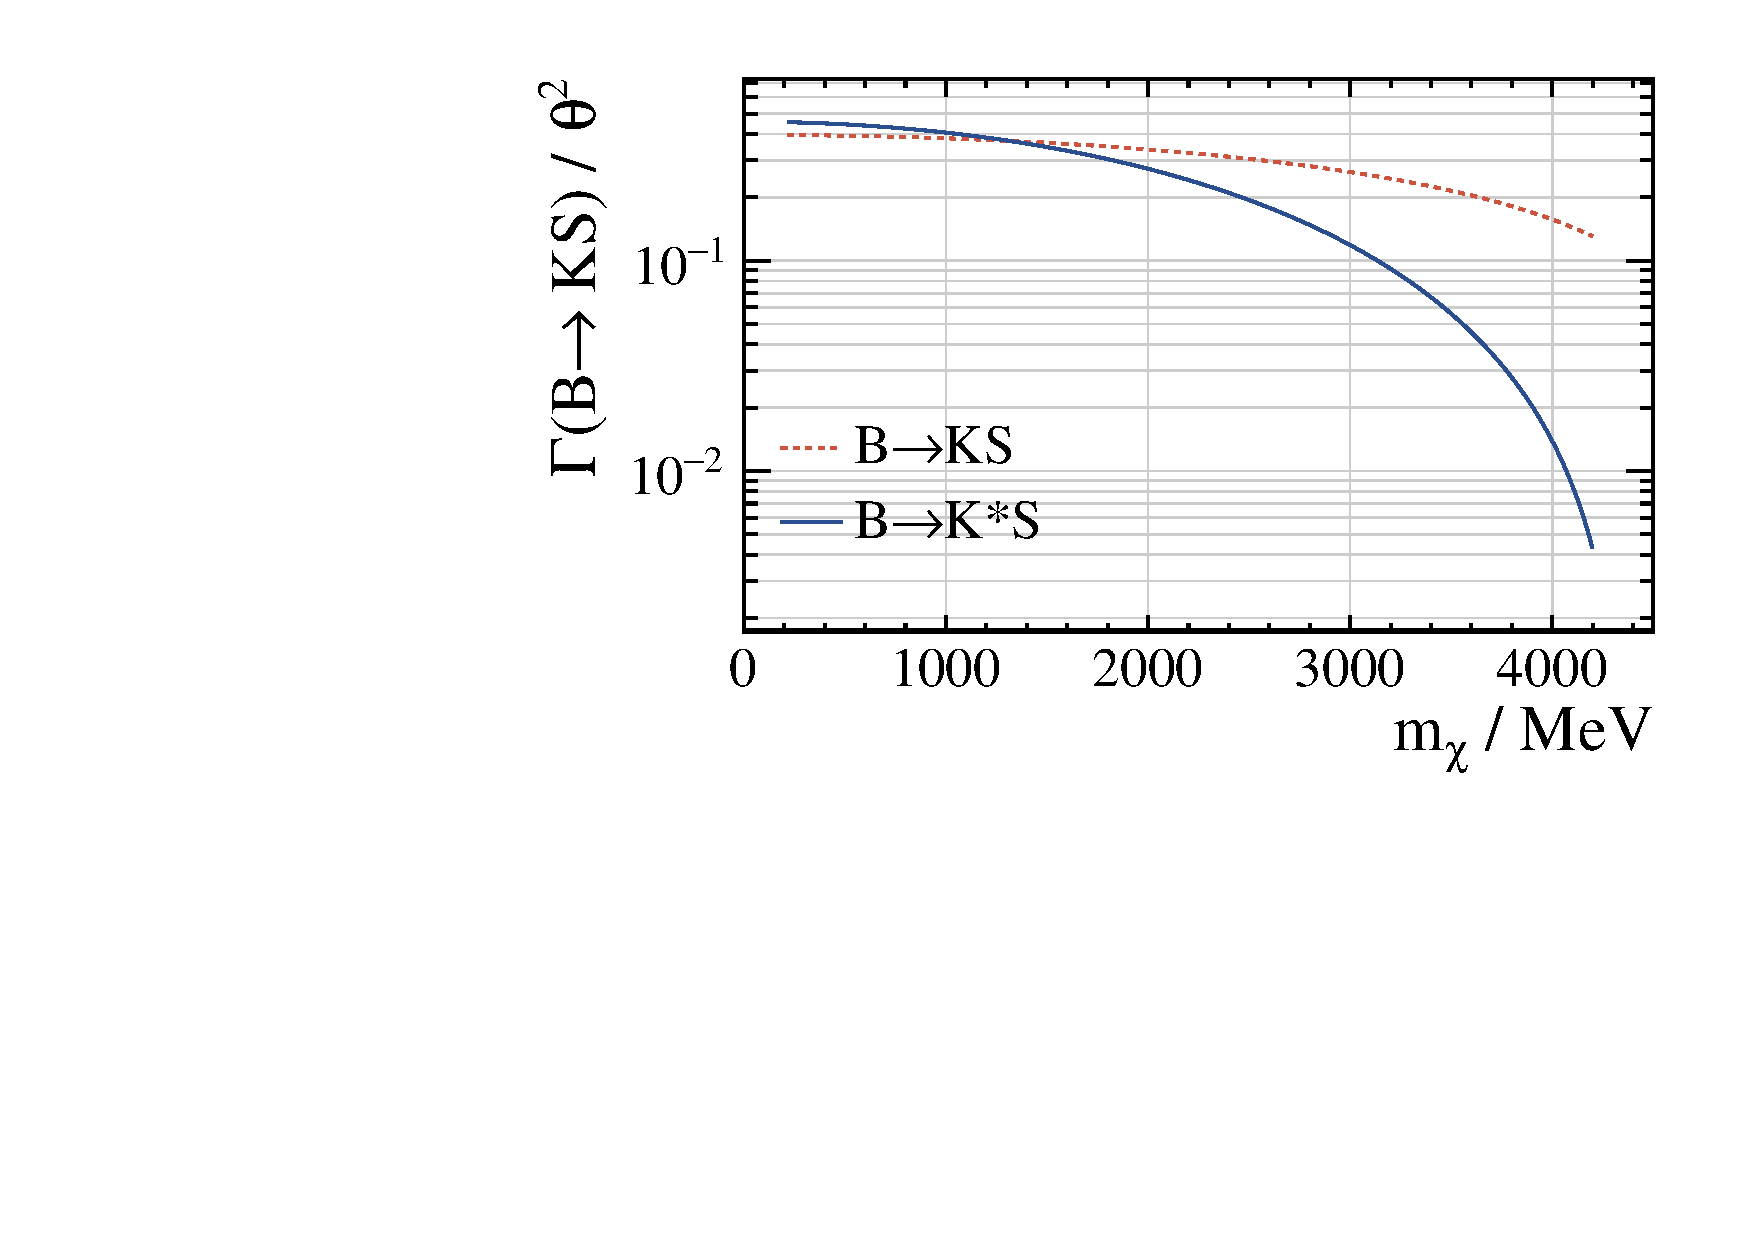
\includegraphics[width=0.48\textwidth]{bf_b2ks_root}
    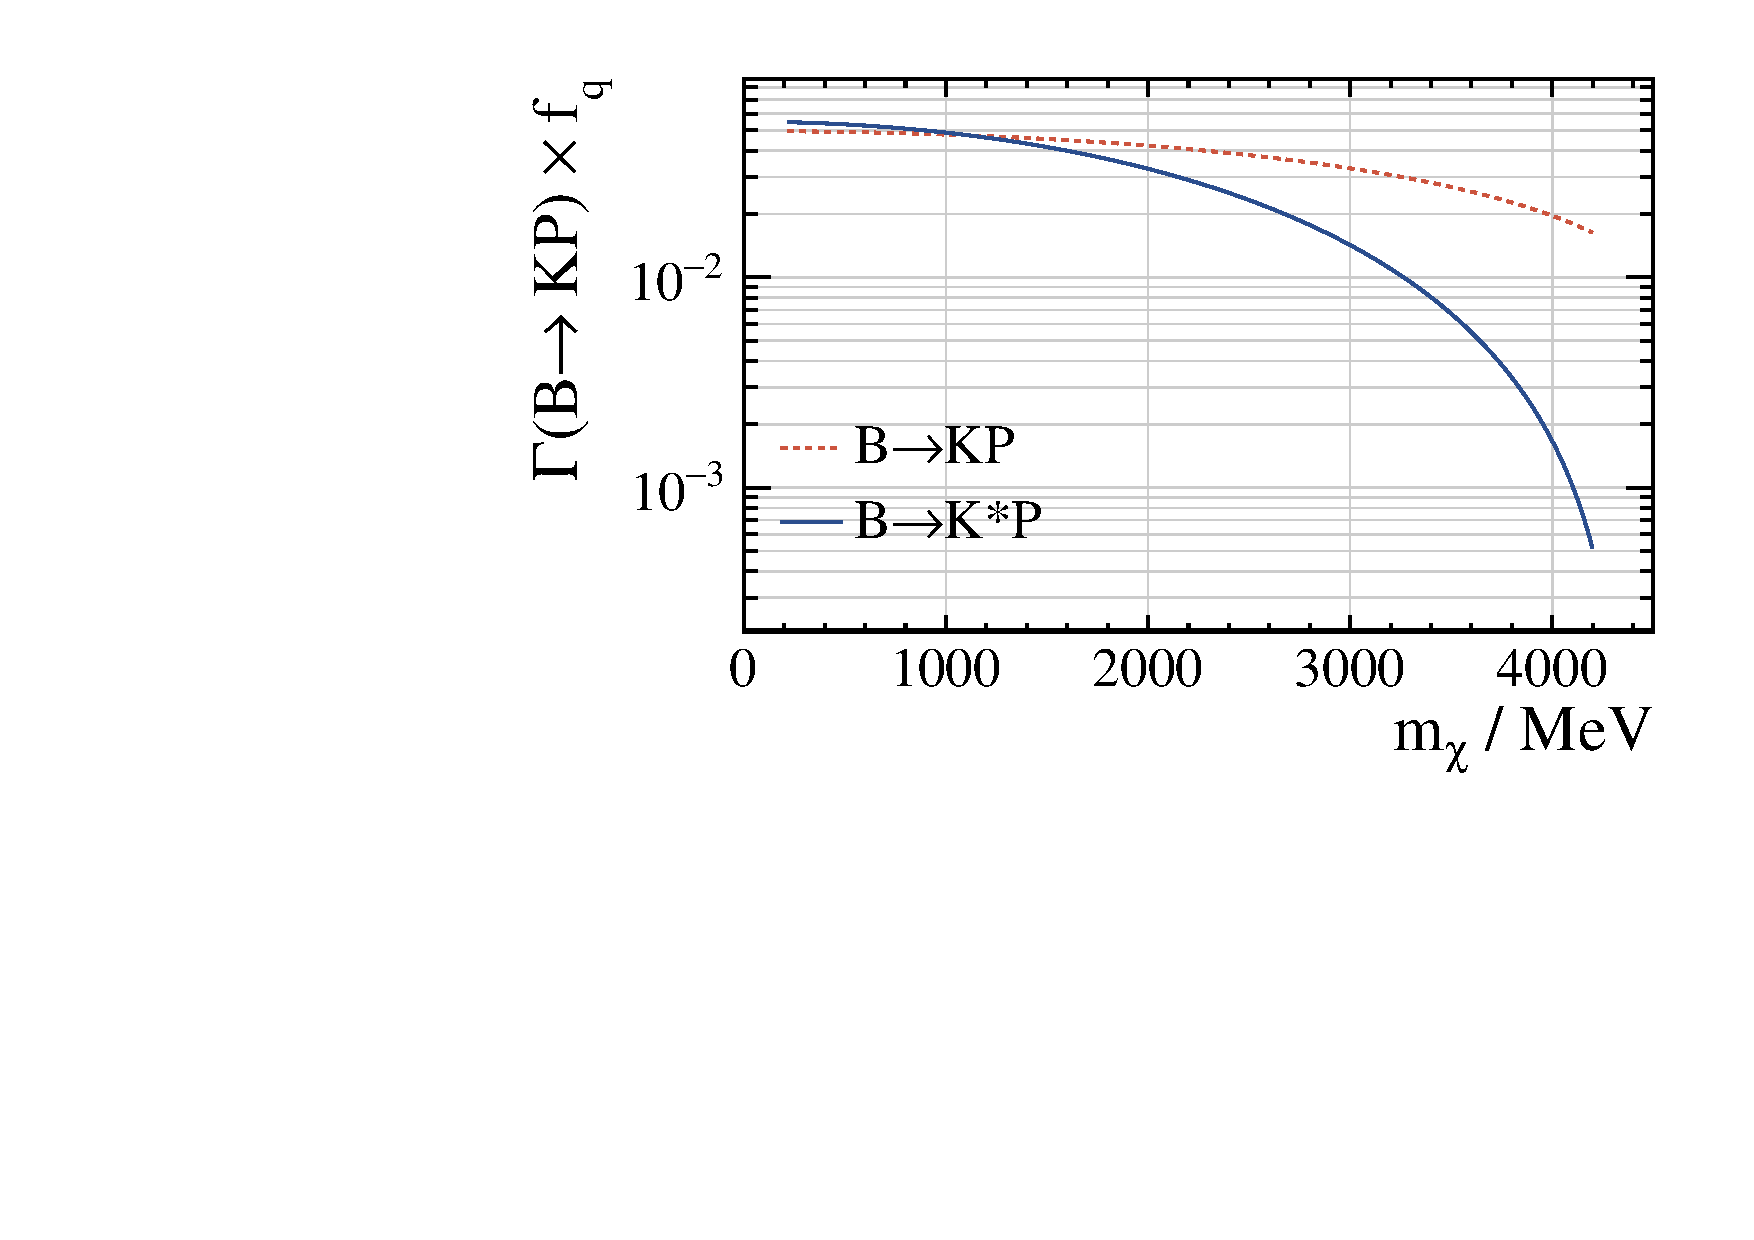
\includegraphics[width=0.48\textwidth]{bf_b2kv_root}
    \caption[Decay rates for decays of the form \decay{B}{K\db}]
    {
      Decay rate predictions, from Eq.~\protect\ref{eq:db:bx},
      for decays of the form $\decay{B}{KX}$, where $X$ is either
      (left) a scalar (S) or
      (right) an axial-vector (P).
      The parameters $\theta$ and $f_q$ are parameters of the model in
      Ref~\cite{Batell:2009jf}.
      The shapes of the curves are dominated by the available phasespace, and sensitivity is
      comparable for $m_\db\lesssim2000\mev$.
    }
    \label{fig:db:kx}
  \end{center}
\end{figure}



The following chapter introduces the analysis strategy, an overview of the selection, and how the
discrete samples of \btokstrdb are used to parameterize various distributions at all masses.
The analysis is performed blindly, some results of the unblinding procedure are given in the final
selection along with a calculated $p$-value.





%Many extensions of the SM predict the existence of a new light boson.
%As all interactions in the SM are gauged, it is reasonable to assume that the same can be said of
%interactions in the dark sector.
%If so, then they would contain new vector bosons such as so-called dark photons (referred to as
%$A^{\prime}$), dark $Z$ bosons (referred to as $Z_d$).
%%A particular model that would anticipate the observation of a light vector boson would one which
%%includes a dark $Z$ (or photon).
%%Such models are motivated by the existence of dark matter and also the $3.6\,\sigma$ deviation
%%exhibited between the theoretical and experimental measurements of the anomalous magnetic moment of
%%the muon, $a_\mu=\tfrac12(g_\mu-2)$~\cite{PDG2012}.
%A $Z_d$ that weakly couples to the visible sector with low mass
%($10\lesssim m_{Z_d}\lesssim500\mev$) would add corrections to the theoretical value of $a_\mu$
%bringing it in line with what is seen experimentally.
%Such models are outlined in Refs.~\cite{Davoudiasl:2012qa,Davoudiasl:2012ag,Lee:2014lga}.
%%Other models might include such particles as Inflatons~\cite{Bezrukov:2009yw} and
%%Axions~\cite{Peccei:2006as}.
%Other models include the Pecci-Quinn axion~\cite{PhysRevLett.38.1440}, as described in \Sec{ch:th},
%which solves the strong \CP problem by the addition of a pseudoscalar axion particle.



%In general, extensions to the SM include bosons that couple to fermions proportionally to
%their masses.
%This occurs either due to mixing with the SM Higgs boson or due to the fact that the
%new bosons arise via a symmetry breaking process similar to the Higgs mechanism.
%Therefore, processes that are mediated via loops that contain top quarks are excellent places to
%search for such particles.



%The spin of the particle is not assumed either.
%A similar analysis might search for a \db in \decay{\Bp}{\Kp\mumu}, where one might expect
%additional sensitivity to scalar particles.
%However, this is not the case.
%Reference~\cite{Batell:2009jf} gives decay rates for decays of the type \decay{B}{K\db} to be:
%\begin{align}
  %\Gamma\big(\decay{B}{K\db}\big) &= \Gamma_0
  %\frac{\lambda_{K}\big(m_{B}^2-m_{K}^2\big)^2}{m_{B}^6}
  %\left[f_0\!\left(m_\db^2\right)\right]
  %\\
  %\Gamma\big(\decay{B}{\Kstar\db}\big) &= \Gamma_0
  %\frac{\lambda_{\Kstar}^3}{m_{B}^6}
  %\left[A_0\!\left(m_\db^2\right)\right]
  %\\
  %\intertext{where the phasespace factor is}
  %\lambda_\kappa &= \left[
    %\left( m_B^2 - m_\db^2 - m_\kappa^2 \right)^2
    %-4m_\db^2m_\kappa^2
    %\right]^\frac12,
    %\label{eq:db:bx}
%\end{align}
%form factors are denoted as $f_0$ $A_0$, and $\Gamma_0$  is a constant.
%Figure~\ref{fig:db:kx} shows that the phasespace factor is the dominant factor in the shape for all
%the decays, and that searching for a particle, \db, in the decays \decay{\Bd}{\Kstarz\db} and
%\decay{\Bp}{\Kp\db} is equally sensitive for $m_\db\lesssim2000\mev$.
%%For example, Fig.~\ref{fig:th:kx} shows how the branching fraction of \decay{\Bd}{\Kstar\db} is
%%expected to vary with the mass of the \db, in comparison to \decay{\Bd}{K\db}.

%\begin{figure}
  %\begin{center}
    %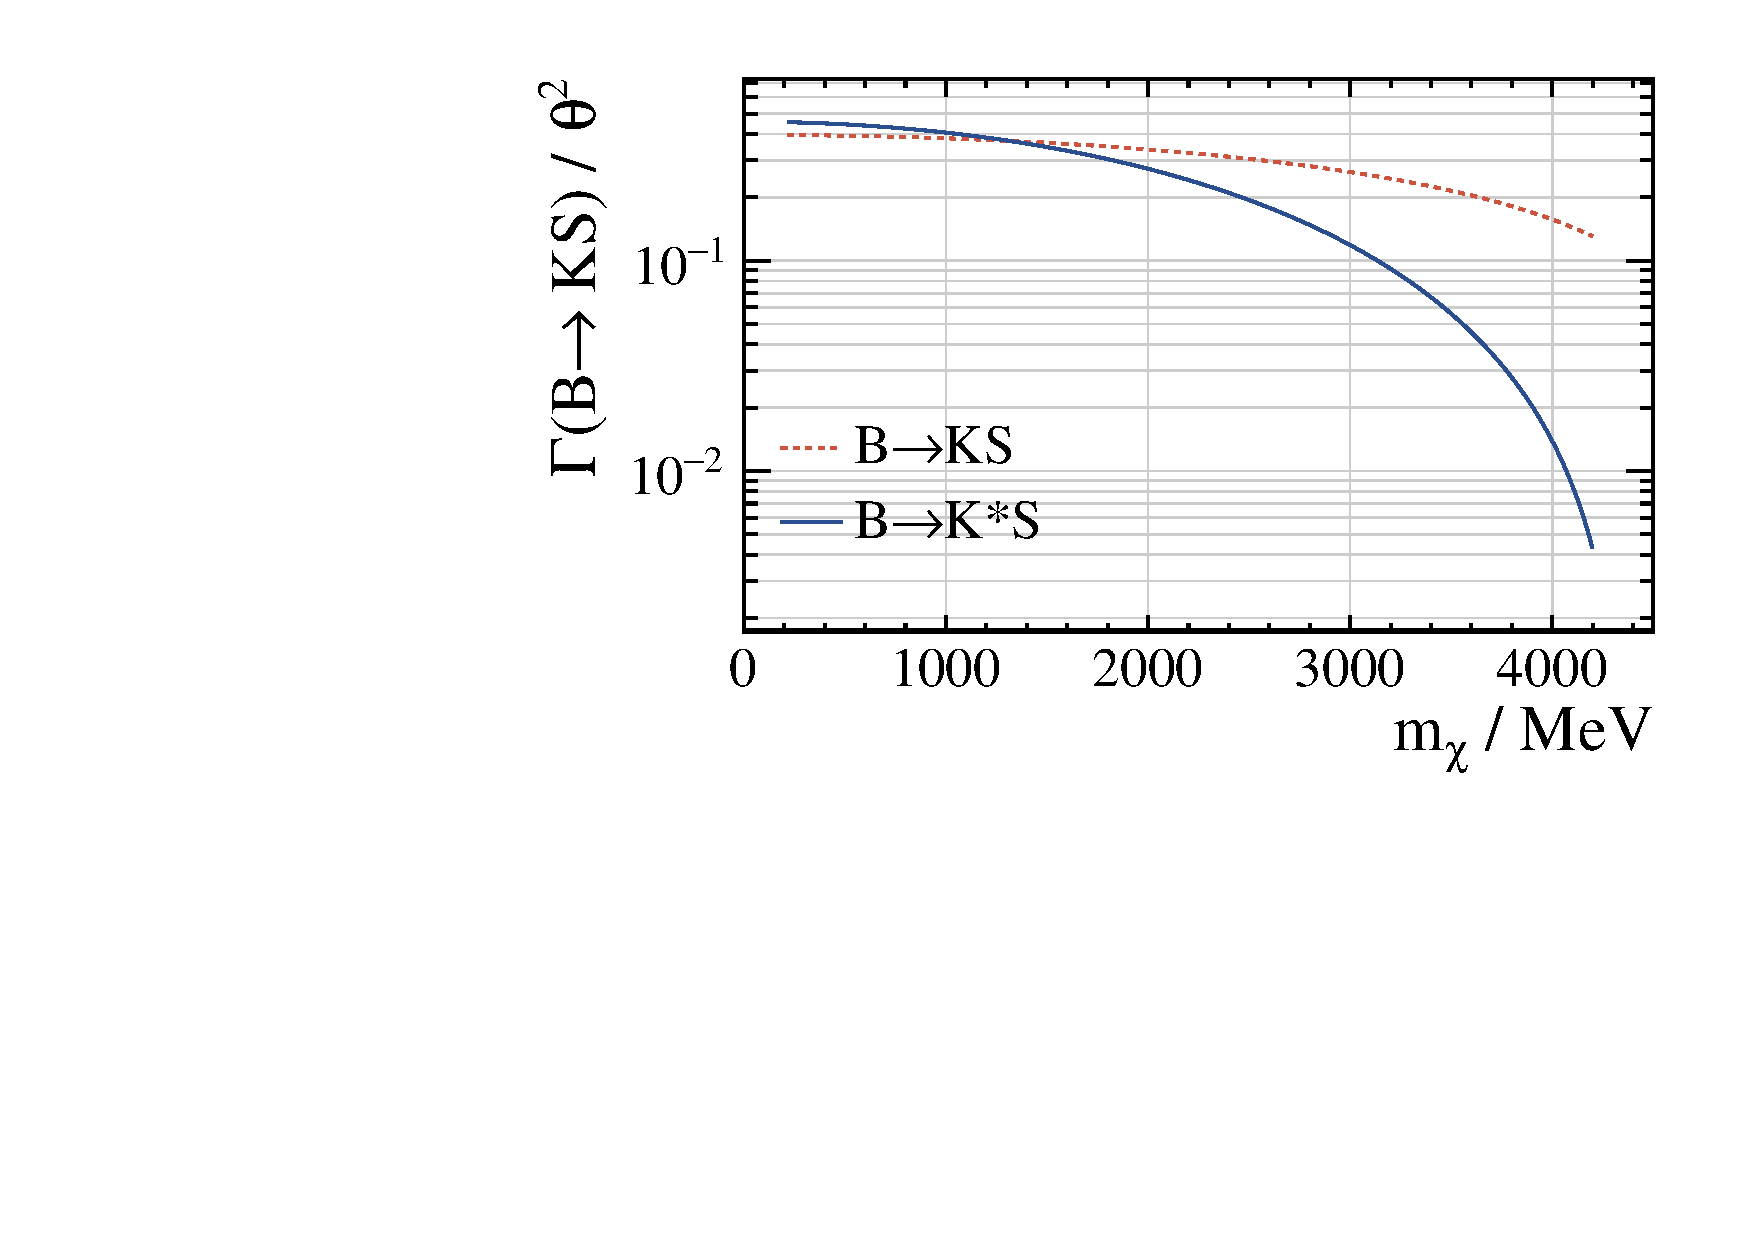
\includegraphics[width=0.48\textwidth]{bf_b2ks_root}
    %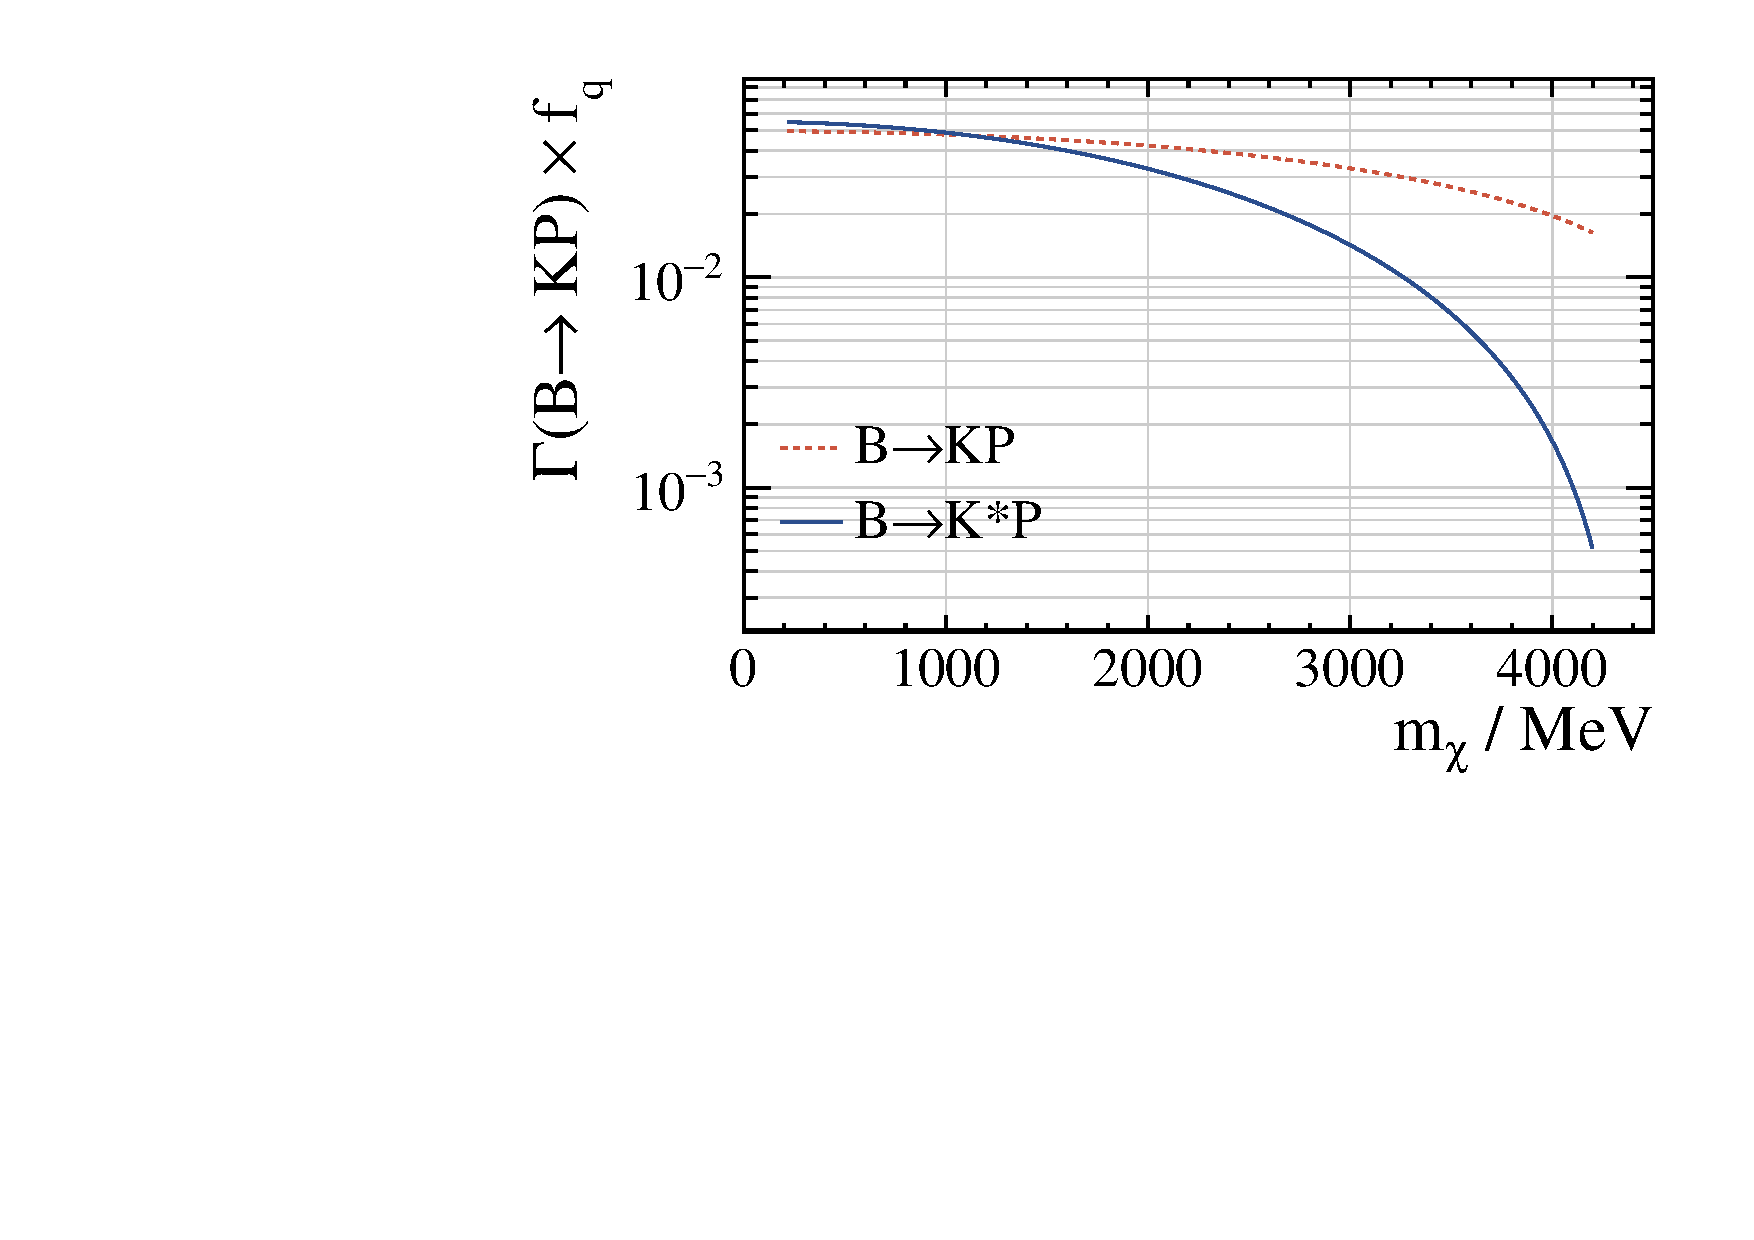
\includegraphics[width=0.48\textwidth]{bf_b2kv_root}
    %\caption{
      %Branching fraction predictions, from Eq.~\protect\ref{eq:db:bx},
      %for decays of the form $\decay{B}{KX}$, where $X$ is either
      %(left) a scalar (S) or
      %(right) a vector (V).
      %The parameters $\theta$ and $f_q$ are parameters of the model.
      %%Note that for these plots $\mathrm{ln}\left(\Lambda_\mathrm{UV}/m_t\right)$ is set to one.
      %The shapes of the curves are dominated by the available phasespace, and sensitivity is
      %comparable for $m_\db\lesssim2000\mev$.
      %%this is taken from Ref~\cite{Batell:2009jf}.
    %}
    %\label{fig:db:kx}
  %\end{center}
%\end{figure}


%The following analysis is a fully frequentist search for a new particle \db, with an unknown mass
%ans lifetime.
%This is done in the two dimensions of mass and lifetime using the method described in
%\Sec{sec:db:strategy}.



%%%%%%%%%%%%%%%%%%%%%%%%%%%%%%%%%%%%%%%%%%%%%%%%%%%%%%%%%%%%%%%%%%%%%%
% NOTHING BEYOND HERE
%%%%%%%%%%%%%%%%%%%%%%%%%%%%%%%%%%%%%%%%%%%%%%%%%%%%%%%%%%%%%%%%%%%%%%
